\chapter{Architecture and Design of \texttt{JHygge}}\label{sec:architecture}

Now that we've discussed the architecture and design of the reference compiler, \texttt{hyggec}, in \ref{sec:hygge_architecture}, we'll attempt to come up with
a refined architecture and design for the new compiler, \texttt{JHygge}. The reason we call it a refined architecture is due to
the fact that \texttt{hyggec} has many good design points for its intended purpose. The design is simple and minimal; very
few types and functions that form a straight-forward pipeline. There are however some less desirable consequences of this.

The design is not very flexible as there is a lot of coupling, some code duplication and deeply nested code. The different
phases depend on concretizations rather than interfaces and they are monoliths; for example, the interpreters \texttt{reduce}
implements the entire set of reduction rules, aside from a few miscellaneous utilities. If a student wants to compare two different
implementation strategies for a while loop, for example, they have to change to overwrite the existing code and then test it,
potentially getting confused along the way. The same principle applies for the typechecker and code generator as well.

So, overall there are a lot of good things that we want to keep. We want to keep the same compiler phases: Lexing/Parsing, Typechecking,
Interpretation and Code Generation. We want to keep the user-friendly CLI and the same kind of testing suite. The things that we
want to change is the implementation language (\texttt{F\#} to \texttt{Java}), the specific build system and parser generator,
the target language (RISC-V assembly to JVM bytecode), and most profoundly, the internal design of the typechecking, interpretation
and code generator phases.

\section{Gradle as an easy-to-use build system}

When using \texttt{F\#}, the \texttt{dotnet} CLI provides a simple build and project management tool which comes by default
with the installation of the \textit{.NET}-platform. In the Java world, the choice is a little more nuanced as there is
no standard build system supplied with an installation of a JDK. There are, however, quite a few choices, with some of the
most popular choices being Apache \texttt{Maven}\cite{maven}, \textit{Gradle}\cite{gradle} and Googles \textit{Bazel}\cite{bazel} built system.

Assuming that the incoming students don't have any experience with any particular build system, it is desirable that the
build system of choice for \texttt{JHygge} is as easy to learn and use to lessen the burden. \textit{Maven} is very
powerful; it uses a declarative approach to specify a project and its build tasks using the Project Object Model (POM,
written in an XML file).
However, it is also quite complicated with concepts like ``Archetypes'', ``Extensions'', workflow, lifecycle and more,
which will be a barrier to entry for students.

\textit{Bazel} is a newer offering from Google, which is meant to be a scalable, multi-platform and multi-language open source
build system. To use \textit{Bazel}, one has to initial a project ``workspace'' and then specify what to build using a \texttt{BUILD}
file written in a Domain-Specific Language (DSL) called \texttt{starlark}. This may sound simple, but we find that there are a few
issues for our case: in every build file, one has to specify all source files explicitly using \textit{Bazel}s own query language,
which is different from that of both \textit{Maven} and \textit{Gradle}. Also, installing \textit{Bazel} itself is quite strange,
as the \textit{Bazel} authors recommend that one uses the \texttt{bazelisk} installation tool, which itself must be installed using
the \textit{Node Package Manager}, \texttt{npm}, which is a tool for \texttt{javascript} packages. So, there are a lot of dependencies
required to install the build tool in the first place. This is likely to confuse students that are not familiar with all of these tools.

Lastly, there is \textit{Gradle}, which as the title of this subsection suggests is our choice of build system. Why?
\textit{Gradle} is easy to install, or rather to not install, as one can simply place a self-containing wrapper inside the project
(\texttt{gradle-wrapper.jar} executable, plus some \texttt{gradlew} wrapper scripts). So, the students don't have to install anything
this way. The \texttt{gradlew} wrapper script provides a CLI similar to that of the \texttt{dotnet} CLI tool. In terms of required
configuration files, \textit{Gradle} requires a \texttt{build.gradle} (or \texttt{build.gradle.kts}) file, where the user can specify
the project metadata, plugins, dependencies and tasks in either the \textit{Groovy} or the \textit{Kotlin} programming language.
This \texttt{build.gradle} file is written in a concise and declarative style, where the \textit{Gradle} framework provides an
easy to use DSL. For version management of dependencies, one can optionally use a \texttt{libs.versions.toml} file to separate
dependency versioning from task specification. That's it, the student won't have to install anything besides Java and they
can build the project in one simple command: \texttt{gradlew build}.

\section{ANTLR4 for parsing}

Similar to \texttt{hyggec}, we want to use a parser generator tool for ease-of-use as the course ``02247'', as well as this
thesis itself, focuses mostly on the later phases of compilation. We have explored two options, \texttt{JavaCC}\cite{javacc} and \texttt{ANTLR4}\cite{antlr4},
which both looked promising initially. We started out using \texttt{JavaCC} as it is quite similar to \texttt{FsLexYacc}\cite{fslexyacc} used by
\texttt{hyggec} in the hope that we could maintain a similar design. This turned out to be disappointing, as the parser file
grew fast when adding language features: before reaching the \texttt{Hygge0} specification, the parser file had grown to 563
lines of code, which by comparison is approximately 89 percent more than the combined 298 lines of code for the lexer and
parser in \texttt{hyggec} (\texttt{Hygge0} branch). However, the worst part was that \texttt{JavaCC} generated invalid java
code for the parser; it couldn't compile and the author was unable to resolve the issue. Upon encountering these issues,
we realised that \texttt{JavaCC} would incur a high degree of complexity as well as a buggy code generation, which will
degrade user experience and increase the maintainance burden.

So, we tried out \texttt{ANTLR4} instead. \texttt{ANTLR4} is quite different from \texttt{JavaCC}; it uses a \texttt{.g4} grammar
file to specify the syntax of the language in a format similar to E-BNF\cite{ebnf}. \texttt{ANTLR4} will then generate a parser that converts
an input stream to an AST of its own. This AST is intended to be consumed by visitors and listeners\cite{antlr4_book}; a visitor will transform and
compute a result from an AST, whereas a listener will only perform some kind of side-effect without returning a result. As we
intend to keep the AST model from \texttt{hyggec}, we can use a visitor to generate \texttt{Node}s and \texttt{Expr}s from the
\texttt{ANTLR4} AST. We will discuss the implementation and its evaluation later. Another bonus benefit is that \texttt{ANTLR4}
is capable of generating parsers in other languages such as \texttt{python}, \texttt{c++} and \texttt{go}. While this doesn't
impact the development of \texttt{JHygge}, one could reuse the \texttt{.g4} grammar file for the base Hygge language if some
students wanted to do a custom project in another language.

\section{A flexible design for the typechecking, interpretation and code generator stages}

As mentioned earlier when high-lighting the weak points of the architecture of the \texttt{hyggec} compiler, the design is inflexible as it
depends on concretizations rather than abstractions. So, we seek a design that is more aligned with the \textit{SOLID} principles
to increase flexibility, extensibility and decoupling. Our proposed solution is that we split up the \texttt{typer}, \texttt{reduce}
and \texttt{codeGen} functions by grouping the expressions of the Hygge language by feature. We then define interfaces that the
different components can depend on.

In figure \ref{fig:jhygge_all_classes} we provide an
overview of the most important classes of \texttt{JHygge} and their internal relations. On its own, this is not enough to explain or proposed design
changes, but is serves as a reference for the classes, interfaces, exceptions, etc. that we will be discussing.

\begin{figure}[H]
\centering
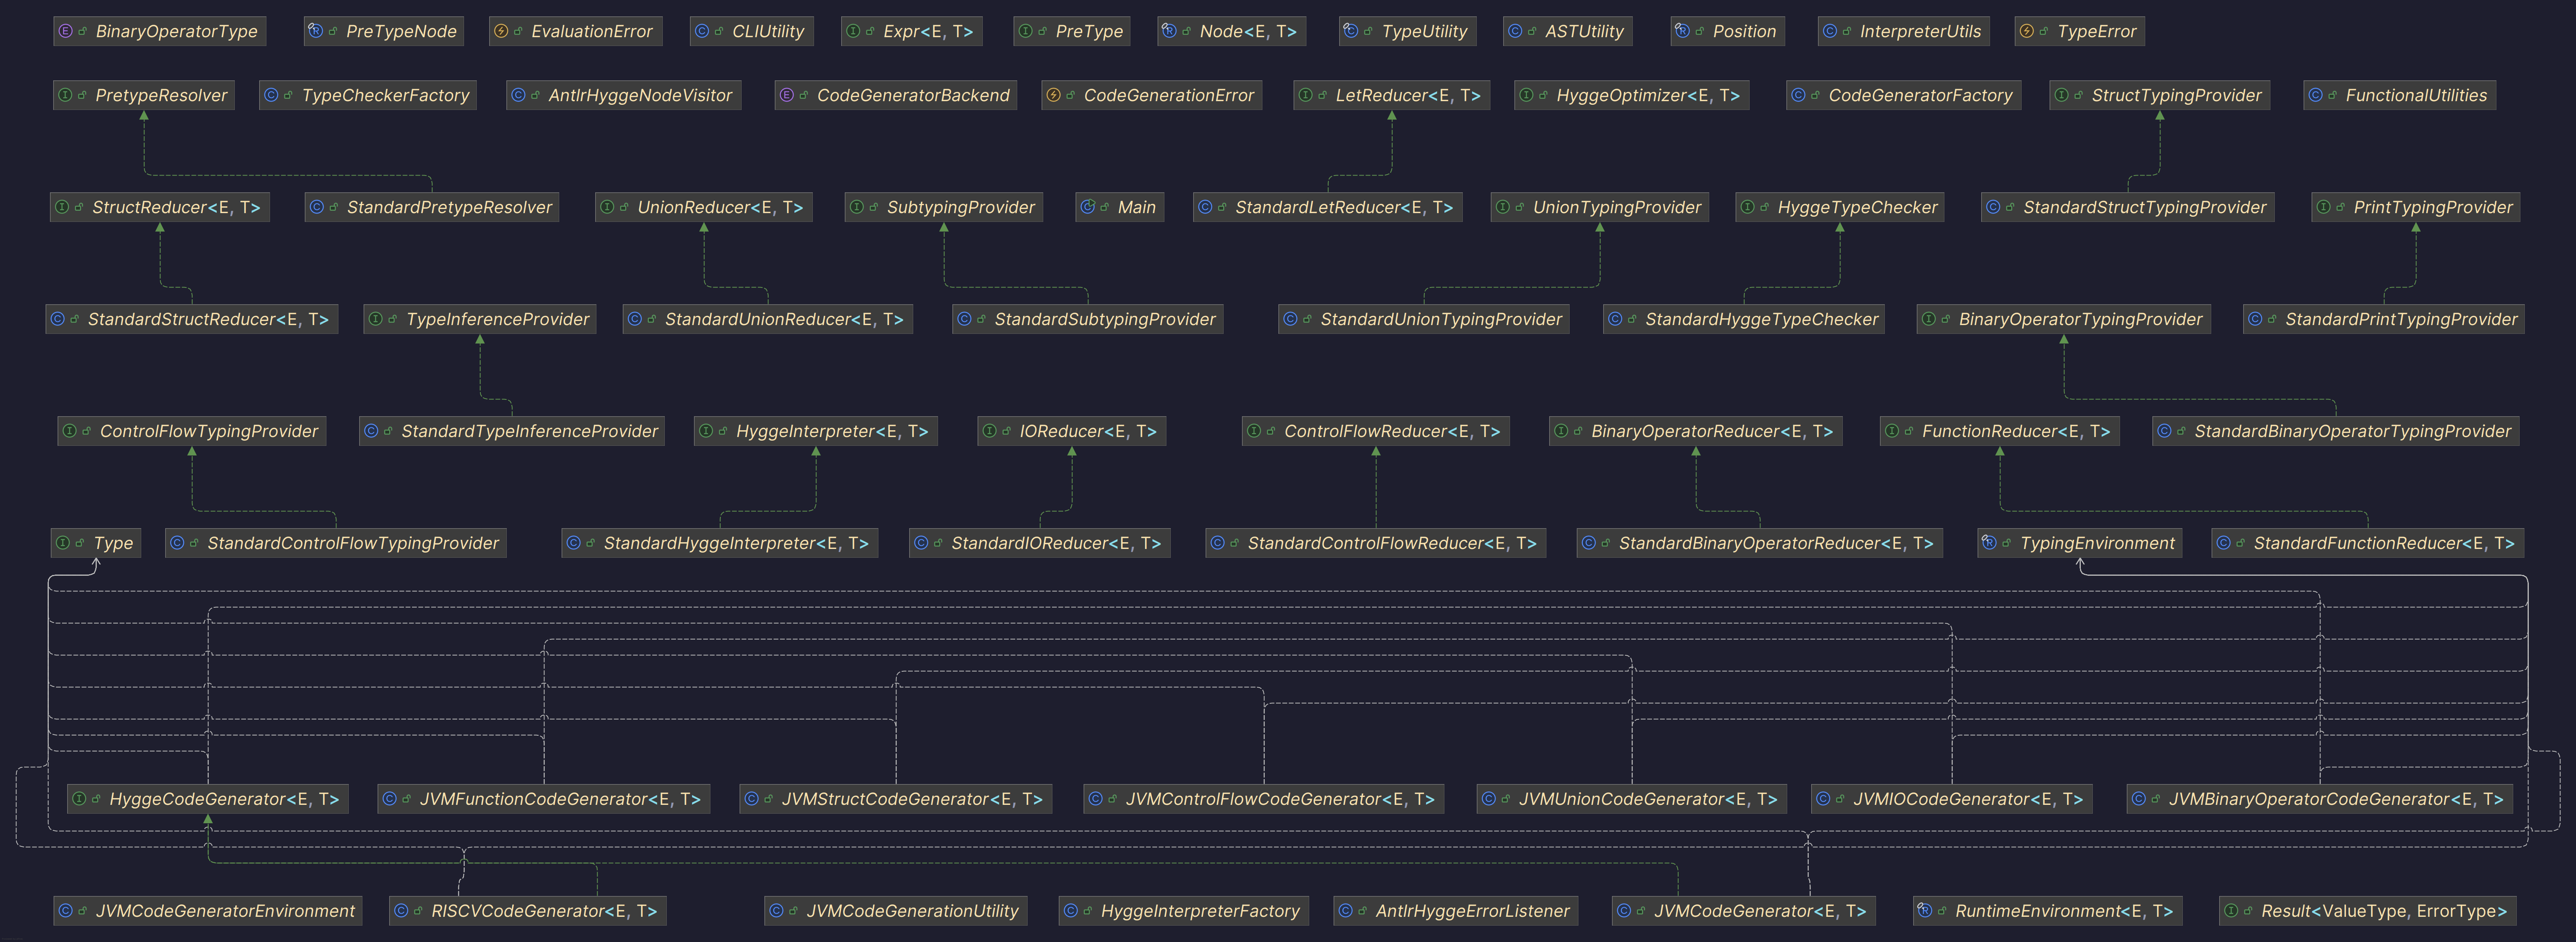
\includegraphics[width=\textwidth]{Pictures/Diagrams/jhygge_all_classes.png}
\caption{All classes of \texttt{JHygge} and their relations. Made using the Diagrams plugin in JetBrains IntelliJ.}
\label{fig:jhygge_all_classes}
\end{figure}

Rather than following the \texttt{hyggec} approach of, for the most part, putting every related function and type in the same source file
for each compiler phase, we have decided to split up each phase into multiple files for a few reasons. Firstly, we assume that the \texttt{Java}
implementation will be lengthier than the \texttt{F\#} one due to \texttt{Java}s presumably more verbose syntax, and it is generally good
practice to put every class, interface, exception, etc. in its own source file. Also, this distribution over multiple files and packages
means that every file will follow the separation of concerns principle and improve rigidity (as defined in ``Clean Code'' by R. C. Martin)\cite{clean_code}. 

Looking solely at the components of the \texttt{ast} package shown in \ref{fig:ast_classes}, it contains almost the same constructs as \texttt{AST.fs} in \texttt{hyggec}, so not much has changed
except for the introduction of the \texttt{ANTLRHyggeNodeVisitor} and the \texttt{ANTLRHyggeErrorListener}, which is due to the dependency on \texttt{ANTLR4}.

\begin{figure}[H]
\centering
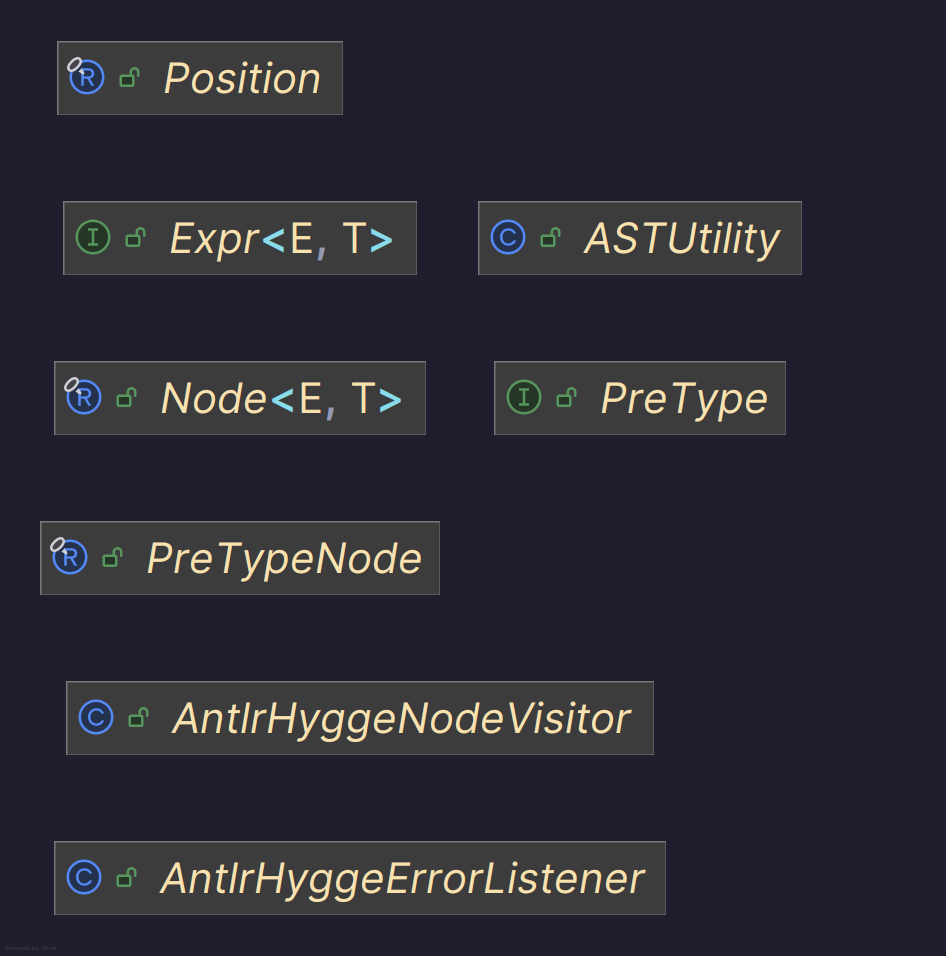
\includegraphics[width=0.7\textwidth]{Pictures/Diagrams/ast_classes.png}
\caption{The classes of \texttt{ast} package in \texttt{JHygge} and their relations. Made using the Diagrams plugin in JetBrains IntelliJ.}
\label{fig:ast_classes}
\end{figure}

In the \texttt{interpreter} is where we begin to see some significant changes in design compared to \texttt{hyggec}; there are interfaces for
every grouping of language features and there is a \texttt{HyggeInterpreterFactory} for creating instances of \texttt{HyggeInterpreter}s.
The important part is that one is no longer intended to directly create concrete instances of some interpreter, that is all handled by
the factory, which also constructs and injects the correct dependencies of the concrete interpreter. This gives the students more flexibility
if they, for example, would want to compare different implementations of the same language feature, they can easily swap between implementations
due to dependency injection and the factory class. Perhaps, the students may want to change the interpretation strategy, so with this design
the students can keep the default interpreter as a reference, while implementing the new strategy incrementally. It is important to note that
from a technical standpoint, this design only requires the programmer to implement the \texttt{HyggeInterpreter}-interface, so the programmer is completely
free to use the remaining interfaces that partially define the interpretation for a grouping of language features. Note also, that there is a
\texttt{standard} package which implements the same interpretation strategy from \texttt{hyggec}.

\begin{figure}[H]
\centering
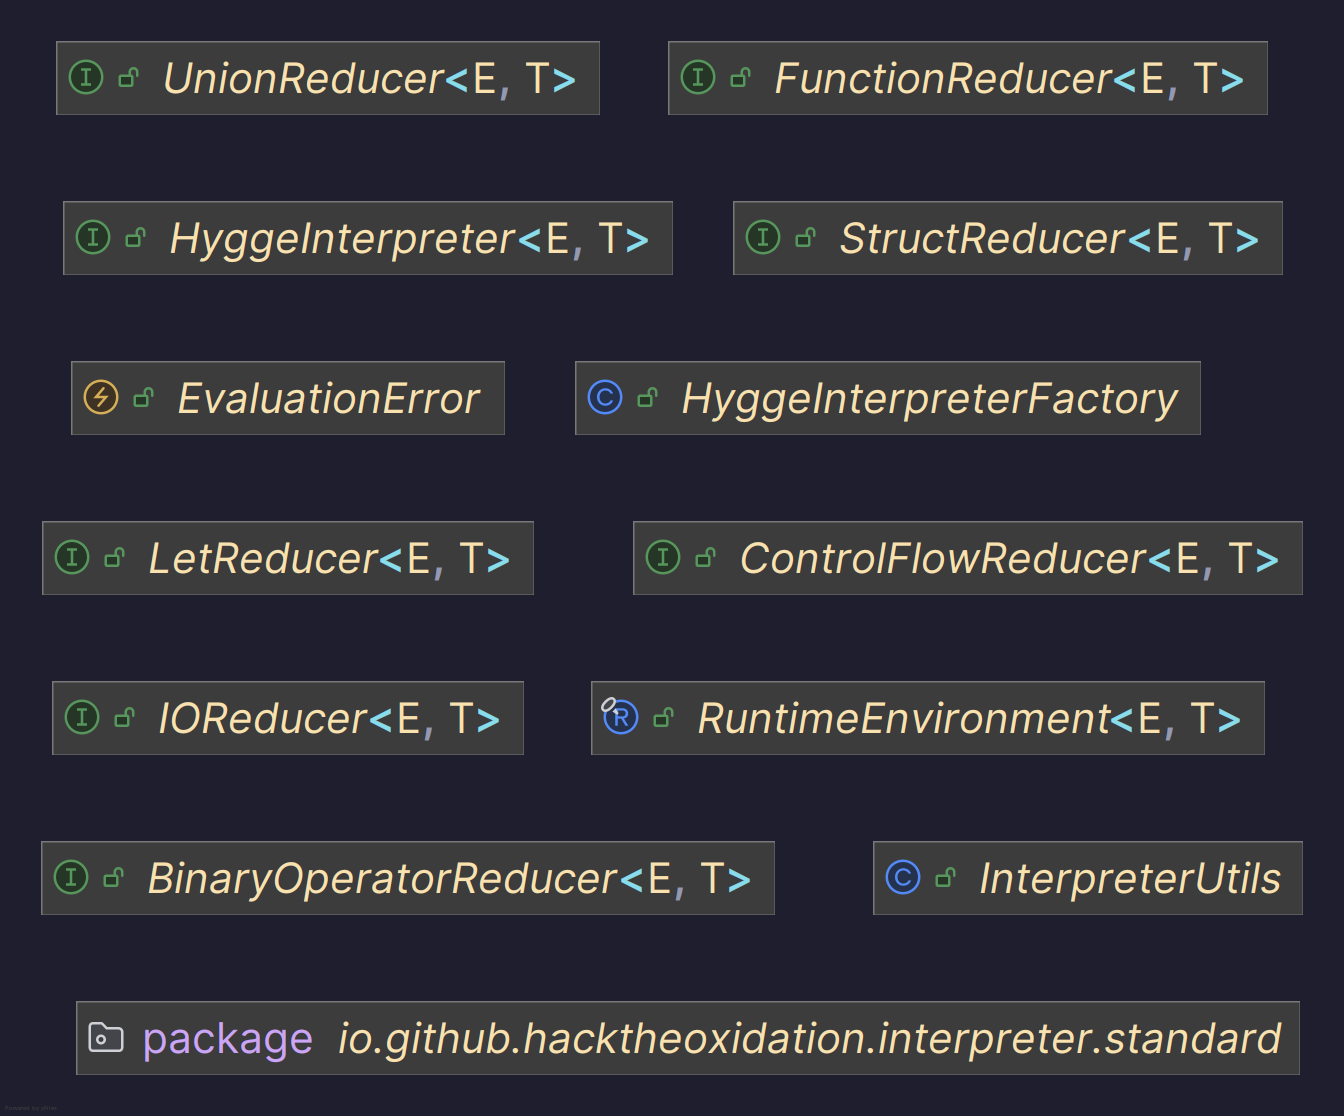
\includegraphics[width=0.7\textwidth]{Pictures/Diagrams/interpreter_classes.png}
\caption{The classes of the \texttt{interpreter} package in \texttt{JHygge} and their relations. Made using the Diagrams plugin in JetBrains IntelliJ.}
\label{fig:interpreter_classes}
\end{figure}

Overall, we repeat this pattern for both the typechecker and the code generator phases as they share the same structure albeit providing different
transformations and effects. On figure \ref{fig:typechecker_classes}, we see the exact same structure and separation of concerns for the typechecker as we saw for the interpreter. 

\begin{figure}[H]
\centering
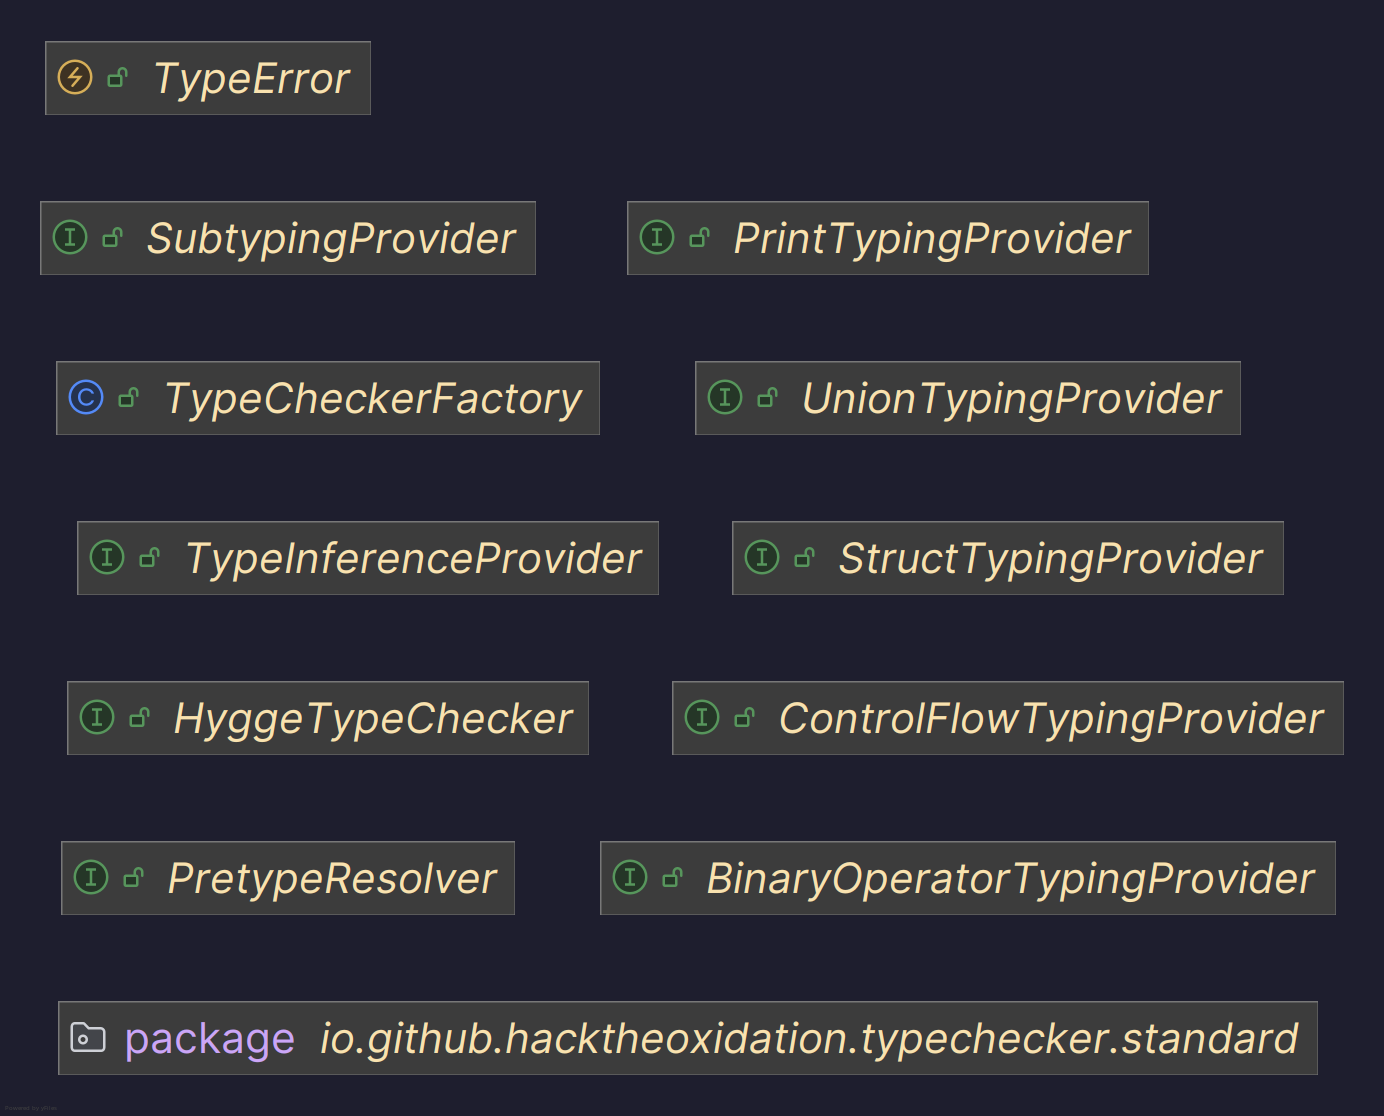
\includegraphics[width=0.7\textwidth]{Pictures/Diagrams/typechecker_classes.png}
\caption{The classes of the \texttt{typechecker} package in \texttt{JHygge} and their relations. Made using the Diagrams plugin in JetBrains IntelliJ.}
\label{fig:typechecker_classes}
\end{figure}

The code generator design is slightly different as shown on figure \ref{fig:codegenerator_classes}. The premise is different to that of the typechecker and interpreter because we don't define
exact rules for the code generation strategy except for the semantics and we expect that there will not only be potentially many code generator backends,
but the target languages of the backend may differ greatly. For example, RISC-V assembly and JVM bytecode are not only different from a syntactic point
of view, but the underlying machines/hardware have almost nothing in common, so it doesn't make sense to try to create some generalized abstractions;
the JVM is stack-based with managed memory\cite{jvm_spec} which isn't the case for RISC-V. By adding another backend, say LLVM IR, this would make generalization
even more difficult. So, rather than coming up with fragile abstractions, we decided to only provide a basic \texttt{HyggeCodeGenerator} interface
along with a factory and then let the programmer decide the best strategy for each backend. There is also a \texttt{jvm} package, which will be
discussed in the following subsection.

\begin{figure}[H]
\centering
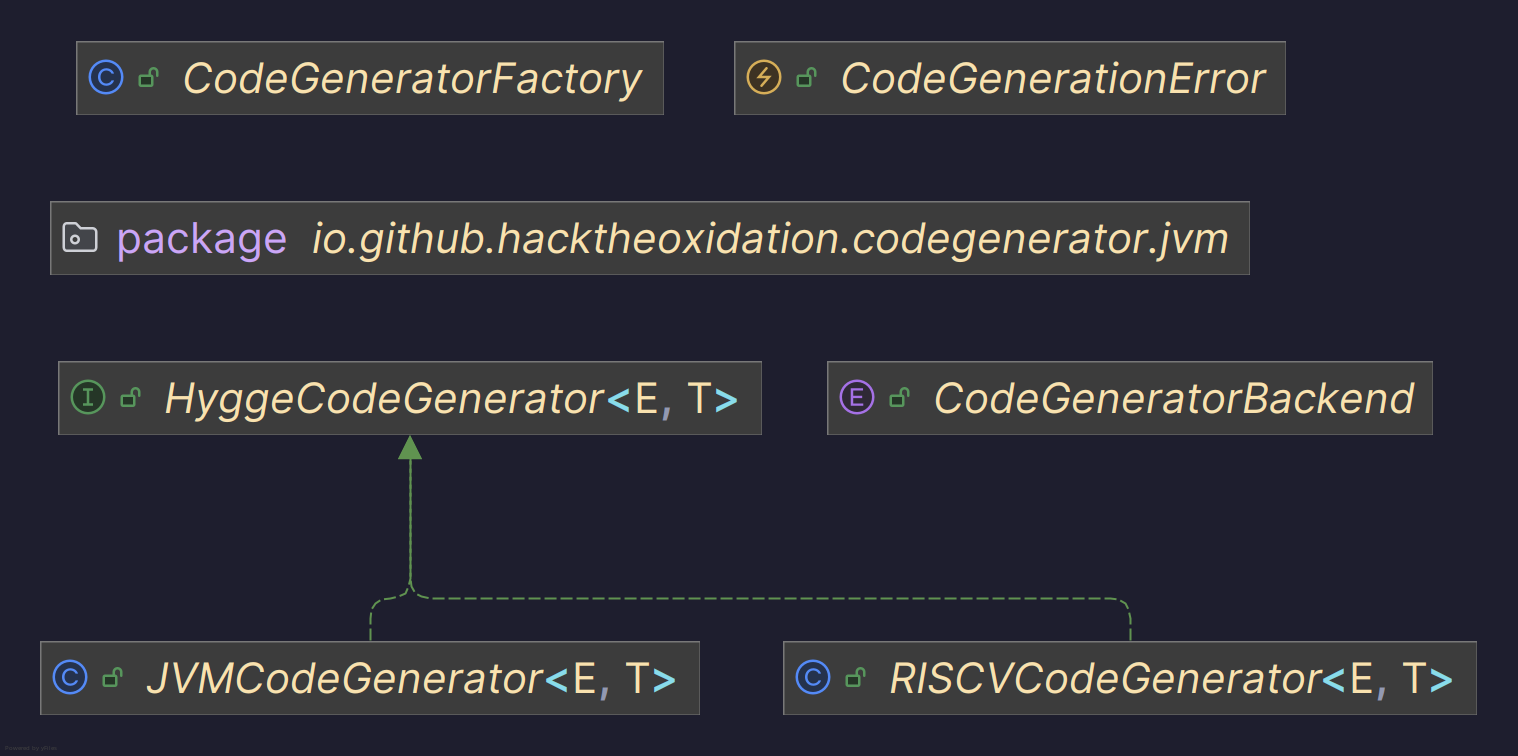
\includegraphics[width=0.7\textwidth]{Pictures/Diagrams/codegenerator_classes.png}
\caption{The classes of the \texttt{codegenerator} package in \texttt{JHygge} and their relations. Made using the Diagrams plugin in JetBrains IntelliJ.}
\label{fig:codegenerator_classes}
\end{figure}

\section{Java 24 Class-file API for JVM bytecode generation}

The \texttt{hyggec} compiler implements its own abstraction layer for RISC-V assembly to ease the implementation of the code
generation phase. This is one the good points about the \texttt{hyggec} compiler, which we want to maintain in the \texttt{JHygge}
compiler. Instead of writing an abstraction layer from scratch, we seek to utilize an existing framework for manipulating JVM
bytecode.

Luckily, there are a few well-maintained frameworks out there. Perhaps, the most interesting framework is the introduction of the
Class-file\cite{jep484} API with the release of Java 24. This is a built-in framework for performing CRUD operations on java `.class`-files
that comes with every JDK from Java 24 onwards. As an alternative, there is the ASM framework\cite{asm}, which is widely used in compilers
and related projects such as OpenJDK, the \textit{Groovy} compiler and the \textit{Kotlin} compiler. While both provide the
same functionality that we seek, the Class-file API has two advantages: it comes with the JDK out-of-box, so there is no
need to manage any additional dependencies, and it has a declarative API which fits in with the function programming style.

As a counter argument, one could say that ASM has seen more real-world use, and that there is nothing wrong with a more imperative
API, but the declarative style employed by the Class-file API and the reduction in the number of external dependencies is very
appealing. As such, we have selected the Java 24 Class-file API as the framework of choice for JVM bytecode generation.

\begin{figure}[H]
\centering
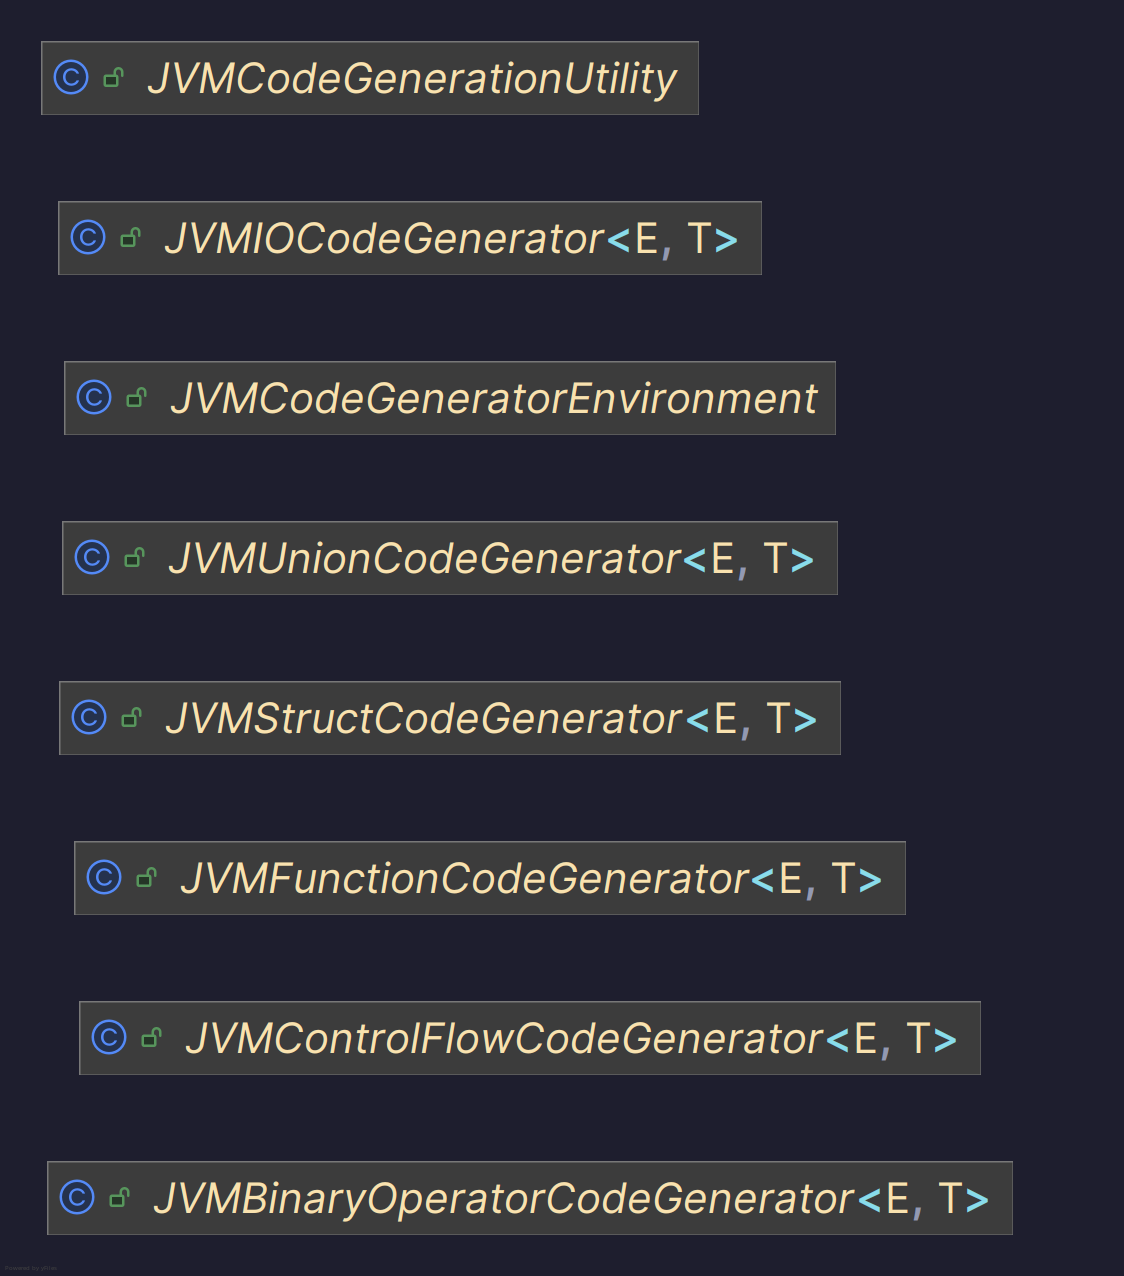
\includegraphics[width=0.7\textwidth]{Pictures/Diagrams/jvm_codegenerator_classes.png}
\caption{Implementation classes of the code generator interfaces for the JVM backend in \texttt{JHygge}. Made using the Diagrams plugin in JetBrains IntelliJ.}
\label{fig:jvm_codegenerator_classes}
\end{figure}

Following our design approach outlined in the previous subsection, we propose a design for the JVM code generation backend to consist of the
classes shown in figure \ref{fig:jvm_codegenerator_classes}. This design still follows the separation of concerns principle, however we have chosen to not make interfaces for everything
as we assume that there will only be one code generation backend for JVM bytecode, where potential improvements will be implemented implace.
This is also due to the fact that the code generation strategies may be very different for different target languages.

\section{PicoCLI for a user-friendly CLI}

The \texttt{hyggec} compiler has a CLI for invoking the different compiler phases on a source file. This is a very useful feature,
when the student want to quickly test an arbitrary hygge program, so we want to maintain a similar CLI in the \texttt{JHygge} compiler.
\texttt{hyggec} uses the \texttt{CommandLineParser}\cite{commandlineparser} library. In the Java world, there is a similar framework called \texttt{PicoCLI}\cite{picocli},
which provides a flexibility in creating a custom commandline argument parser for multiple different JVM languages. This project
is well maintained and is used by some of the Apache projects, like \texttt{Groovy}, \texttt{Hive} and \texttt{Hadoop}, at the time of writing.
